
%(BEGIN_QUESTION)
% Copyright 2010, Tony R. Kuphaldt, released under the Creative Commons Attribution License (v 1.0)
% This means you may do almost anything with this work of mine, so long as you give me proper credit

A DDC (Direct Digital Control) system used for building automation sends a 4-20 mA control signal to a steam valve with an electronic positioner.  This particular loop has a problem, for the valve remains in the full-closed (0\%) position regardless of what the DDC tries to tell it to do.  A technician begins diagnosing the problem by taking a DC voltage measurement at terminal block TB-11 in this loop circuit:

$$\includegraphics[width=15.5cm]{i00717x01.eps}$$

The technician knows a reading of 22.6 volts indicates an ``open'' fault.  Based on the location of the measured voltage (22.6 VDC), determine where in the wiring a single ``open'' fault could be located.

\vskip 10pt

For the next diagnostic test, the technician momentarily connects a jumper wire between the screws of TB-10 while continuing to measure voltage at TB-11.  The new voltage measurement at TB-11 (with the jumper installed) reads 0.0 volts.  Determine what this result tells us about the nature and location of the fault.

\vskip 10pt

Explain whether or not there is any danger of introducing a short-circuit into a system like this.  Could a fuse be blown by doing this test?

\vskip 20pt \vbox{\hrule \hbox{\strut \vrule{} {\bf Suggestions for Socratic discussion} \vrule} \hrule}

\begin{itemize}
\item{} Explain why it is critically important to determine the identities of the valve and DDC card as being either electrical {\it sources} or electrical {\it loads} when interpreting the diagnostic voltage measurements.
\item{} Identify some of the pros and cons of this style of testing (measuring voltage at a set of points before and after a purposeful wiring short) compared to other forms of multimeter testing when looking for either an ``open'' wiring fault.
\item{} Describe a good ``next test'' to perform on this system to further diagnose the location and nature of the fault.
\end{itemize}

\underbar{file i00717}
%(END_QUESTION)





%(BEGIN_ANSWER)


%(END_ANSWER)





%(BEGIN_NOTES)

Based on the first measurement (only), we could conclude the wiring fault {\it may} be an ``open'' in either cable 30 or in cable 41.

\vskip 10pt

After taking the second measurement, we must conclude the fault is an ``open'' in cable 41 (or an ``open'' fault in the valve positioner).
\vskip 10pt

There is no danger in introducing a short into the system, because the DDC's 4-20 mA output is naturally current-limited like all 4-20 mA output channels.

%INDEX% Troubleshooting review: electric circuits

%(END_NOTES)


